\section{Control Circuit}
%TODO James to update with his design

For this project we chose an accelerometer from Freescale Semi (FXLN8361QR1) which operated between 1.7\,V and 3.6\,V. The device can also toggle between a low sensitivity mode ($\pm8g$) and a high sensitivity mode ($\pm2g$). When the power is supplied and mode set, the accelerometer outputs three voltages proportional to the acceleration in X, Y, and Z.

Thus on level ground at rest, the accelerometer should measure a net acceleration of $[0,0,-g]$. However, at zero acceleration, the device outputs an offset voltage of 0.75\,V, thus the equilibrium position in terms of voltage will be $[0.75\,V,0.75\,V,0.979\,V]$.

The control circuit uses the output of our accelerometer to provide power to the motors with the intent of either stabilizing or moving our quad-copter. This means that the control circuit must have six outputs to move our device in a three-dimensional Cartesian coordinate system. To move the device up or down in the Z direction, the output must be connected to all four motors; however, to move the device in the X or Y directions, the outputs must be connected to only two motors at a time, using diodes to determine the relative voltage given to each motor pair. 

For our initial design, we have chosen to only allow movement in the Z direction, with the intent of incorporating the X and Y directional movement at a later date (Figure ~\ref{fig:ctrl}). The circuit, itself, first uses a differential amplifier to compare the output of the accelerometer to the equilibrium positions, 0.75\,V, 0.75\,V, 0.979\,V for X, Y, and Z respectively. Then it integrates the difference between the acceleration in each direction and its equilibrium position and compares that value with another differential amplifier to a voltage provided by the user. In order to stabilize the X and Y directions, this signal has been set to ground for those directions. At this point, it is entirely possible that the signal is negative, so we split the signal with a pair of diodes and if the signal is negative, we sent it through an inverting amplifier before going to the motor control circuit.

There are a few restrictions on this circuit. The output must be between 2.4 and 6 V for the motor control circuit and the op amps require negative voltage. The former will be require some testing after characterizing our motors (Appendix A). The latter can be solved by creating negative signal from a positive source with a switch.

%To determine this equilibrium, we need to integrate the Z signal twice to determine the net displacement, and select for the height we wish to hover at with a comparator. Then to balance, we also integrate both X and Y signals once to select for zero velocity. Since the comparator will output a rail voltage based on the net difference between measured value and set point, it must be scaled to appropriately control the motors to restore balance.

\begin{figure}[h]
	\centering
	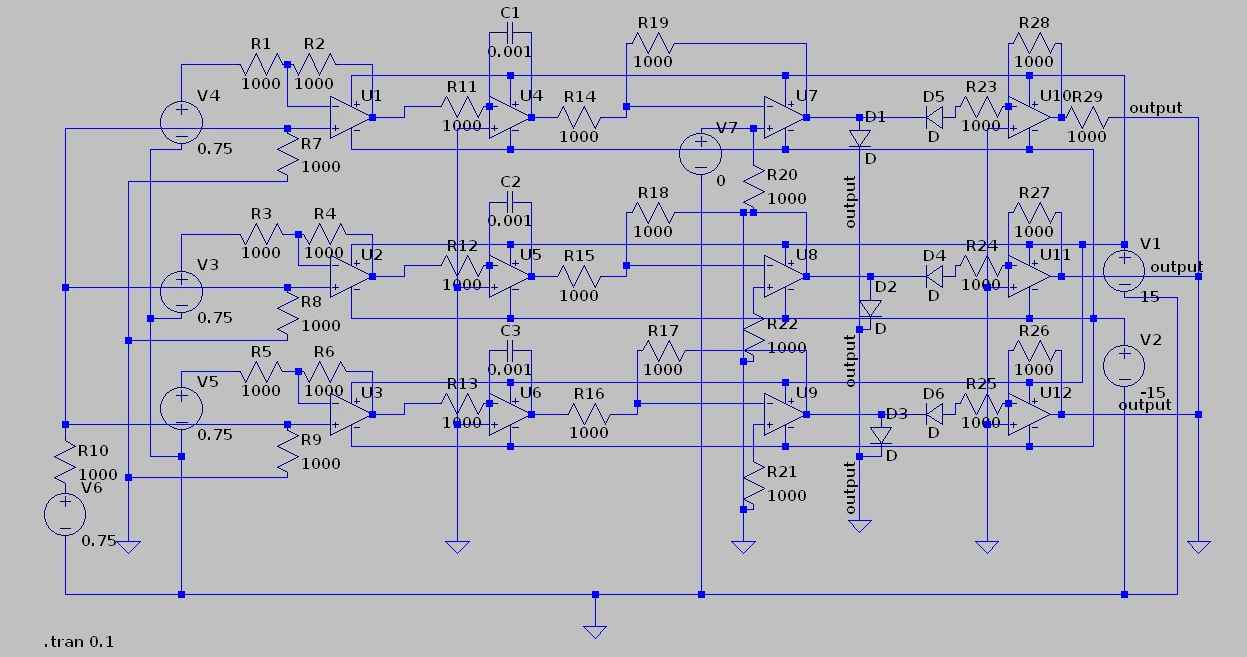
\includegraphics[width=\textwidth]{ctrl.jpg}
	\caption{Schematic of the control circuit, consisting of a differential amplifier, an integrator, a seconf differential amplifier and an inverting amplifier for the X, Y, and Z outputs of the accelerometer.}
	\label{fig:ctrl}
\end{figure}
